% !TEX root = Projektarbeit.tex

\chapter{Das Kernelmodul - Geräteunabhängige Grundfunktionen} 
Am Beispiel des Treibers für das Waveshare e-Paper-Display sollen nun der Aufbau und die prinzipielle Funktionsweise eines Linux-Treibers sowie auftretende Probleme bei der Umsetzung erläutert werden. 

Im ersten Teil sollen die grundlegenden Funktionen und üblichen Schnittstellen eines Kernelmoduls anhand des Waveshare Treibers genauer betrachtet werden, während sich der zweite Teil auf die hardwarespezifische Implementierung für das Display konzentriert.


\subsection{Kernelspace - eine Vorwarnung}
Zu beachten ist, dass die C-Standardbibliothek im Kernel nicht zur Verfügung steht. Viele oft benötigte Funktionen werden allerdings als leicht gewichtigere Funktionen angeboten. Ebenso gibt es keinen Speicherschutz wie zwischen Anwendungen im Userspace. Fehler in einem Modul können sich auf den gesamten Kernel auswirken und diesen zum Absturz führen. 

\subsection{Debugging}
Debugging ist im Kernel nicht ohne weiteres möglich. Debugger, wie aus modernen IDEs für viele Programmiersprachen bekannt, gibt es so nicht. Dem am nächsten kommt der Kerneldebugger \texttt{kgdb}, der es möglich macht, auf Hochsprachenniveau Kernelcode zu betrachten. Allerdings sind dazu zwei Rechner mit einem komplexen Aufbau nötig, es dauert sehr lange bis der noch experimentelle \texttt{kgdb} lange Symbollisten auflöst und noch nicht alle Hardwareplattformen werden unterstützt. %TODO Kernelbuch S 42
Im Rahmen dieser Arbeit wird daher auf die im Kernel alt hergebrachte Art der Fehlersuche mit \texttt{printk} gesetzt, das mit \texttt{printf} in der C-Standardbibliothek vergleichbar ist. Über \texttt{printk} können mit einer Priorität versehene Kernellogs geschrieben werden, die sich beispielsweise mit \texttt{dmesg} auslesen lassen. An relevanten Stellen lassen sich so Ausgaben, zum Beispiel von Variablenwerten generieren. Um nicht bei jeder Debug-Ausgabe eine Priorität setzen und ein Kürzel für das eigene Modul einfügen zu müssen, wird im Treiber hierfür zuerst ein Makro (Listing \ref{lst:debugmacro}) definiert:

\begin{listing} [H]
\caption{Debug-Macro}
\label{lst:debugmacro}
\begin{minted} [xleftmargin=18pt, breaklines, frame=lines, framesep=2mm, fontsize=\footnotesize, linenos] {c}
#ifdef DEBUG
#define PRINT(msg) 	do { printk(KERN_INFO "waveshare - %s \n", msg); } while (0)
#endif
\end{minted}
\end{listing}

\section{Das Grund-Modul - {\_\_}init und {\_\_}exit}
Ein minimales Modul braucht nicht viel mehr als eine \mintinline{c}{__init}, eine \mintinline{c}{__exit} Funktion und ein Macro, dass dessen Lizenz angibt. Nur Module, die einer Form der GPL\footnote{GNU General Public License; verlangt, dass jedes Programm das in irgendeiner Art und Weise von einem unter GPL lizenzierten Programm abgeleitet wird selbst unter diese Lizenz gestellt und offengelegt werden muss} unterliegen, können den vollständigen Umfang der Funktionen des Linux-Kernels benutzen. %TODO Kernelbuch S. 65
Die \mintinline{c}{__init} Funktion wird aufgerufen, sobald das Modul mit \mintinline{bash}{insmod} oder \mintinline{bash}{modprobe} zum Kernel hinzugeladen und so gestartet wird. Sie initialisiert den Treiber und ist abzugrenzen von der \mintinline{c}{probe} Funktion, die normalerweise dazu genutzt wird nach der grundlegenden Treiberinitialisierung hardwarespezifische Bestandteile des Treibers anzulegen. 
Die \mintinline{c}{__exit} Funktion wird aufgerufen, wenn der Treiber entladen werden soll. Alle Initialisierungen und Reservierungen, vor allem reservierter Speicher müssen freigegeben werden. 

\subsection{Init des Waveshare e-Paper-Treibers}
Der Name der Init-Funktion ist frei wählbar. Über das Macro \\ 
\mintinline {c}{module_init(waveshare_init);} wird  definiert, dass hier die parameterlose Funktion mit dem Namen \texttt{waveshare\_init} und dem Rückgabetyp \texttt{int} verwendet werden soll. 

Die Initialisierung beginnt mit der Anforderung von Gerätenummern für ein Character basiertes Gerät, die dazu genutzt werden den zugehörigen Treiber zu identifizieren sowie die einzelnen Geräte auseinander zu halten. Sie lösen das Konzept von Major-Nummer (Treiberidentifikation) und Minor-Nummer (Geräte auseinander halten) ab und sind in der Lage mehr physikalische bzw. logische Geräte zu unterscheiden. Gerätenummern und Major-/Minor-Nummern können in einander überführt werden. Zur Anforderung der Gerätenummern wird die Funktion \mintinline{c}{alloc_chrdev_region()} (Listing \ref{lst:waveshare_init}, Zeile 15) verwendet. Dabei gibt der erste Parameter eine Referenz auf eine Struktur vom Typ \texttt{dev\_t} (eine Gerätenummer) an. Dort wird die erste angeforderte Nummer abgelegt. Mit dem zweiten wird angegeben bei welchem Wert die Minor-Nummern starten, mit dem dritten, wie viele verschiedene Geräte unterschieden werden sollen. Der letzte Parameter gibt den Namen des Treibers an, der mit der Gerätenummer assoziiert wird. Dabei wird der Treiber für das Gerät beim Kernel angemeldet. Im Fehlerfall springt das Programm zur Sprungmarke \mintinline{c}{free_device_number}. Die Fehlerbehandlung wird im Folgenden näher erläutert.

Mit \mintinline{c}{cdev_alloc()} wird Speicher für ein Objekt des Typs \mintinline{c}{struct cdev *} alloziert, durch das der hier benötigte zeichenorientierte Gerätetreiber repräsentiert wird. Wird hier nicht der geforderte Pointer auf das instantiierte Objekt zurückgegeben, wird die Fehlerbehandlung bei der Sprungmarke \mintinline{c}{free_device_number} begonnen. 

Dem nun angelegten Treiberobjekt, in C durch ein \texttt{struct} repräsentiert, wird im Element \texttt{owner} der Besitzer des Treiber mitgeteilt. Im Element \texttt{ops} wird ein Verweis auf die \mintinline{c}{struct fileoperations} angegeben. In dieser \texttt{struct} (Listing \ref{lst:waveshare_init}, Zeile 1) sind Pointer auf Funktionen gespeichert, die Interaktion des Treibers mit dem Betriebssystem zur Verfügung stellen. Darunter fallen beispielsweise Funktionen zum Öffnen einer Treiberinstanz, Daten aus dem Treiber auslesen, Daten an den Treiber senden, sowie für das Schließen (Freigeben).  

Anschließend wird mit \mintinline{c}{cdev_add(waveshare_obj, waveshare_dev_number, 1)} das instantiierte Treiberobjekt (\texttt{waveshare\_obj}) beim Kernel registriert. Mit \\
\texttt{waveshare\_dev\_number} wird die erste Gerätenummer angegeben, mit der Zahl, wie viele Gerätenummern mit dem Treiber verwaltet werden sollen. 

Bevor nun auf den hardwarespezifischeren Teil der \texttt{init}-Methode eingegangen wird, sollen zuerst die weiteren grundlegenden Treiberbestandteile betrachtet werden. 


\begin{listing} [H]
\caption{waveshare\_init}
\label{lst:waveshare_init}
\begin{minted} [xleftmargin=18pt, breaklines, frame=lines, framesep=2mm, fontsize=\footnotesize, linenos] {c}
static struct file_operations fops = {
	.owner = THIS_MODULE,
	.open = waveshare_driver_open,
	.release = waveshare_driver_close,
	.read =  waveshare_driver_read,
	.write = waveshare_driver_write,
 	.poll = waveshare_driver_poll, 
};


static int __init waveshare_init (void) {

[...]

	if (alloc_chrdev_region (&waveshare_dev_number, 0, 1, WAVESHARE) < 0 ) {
		goto free_device_number;
	}
	
	waveshare_obj = cdev_alloc();

	if (waveshare_obj == NULL) {
		goto free_device_number;
	}

	waveshare_obj->owner = THIS_MODULE;
	waveshare_obj->ops = &fops;

	if (cdev_add (waveshare_obj, waveshare_dev_number,1)) {
		goto free_cdev;
	}

[...]
	
}
\end{minted}
\end{listing}

\subsection{Fehlerbehandlung bei Initialisierungen}
Wie schon erwähnt wird die Fehlerbehandlung bei Treiberinitialisierungen im Kernel über \texttt{goto} Sprungmarken realisiert. Während \texttt{goto}s in der Applikationsprogrammierung nicht gerne gesehen sind, sind sie im Kernel für das Aufräumen in der korrekten Reihenfolge im Fehlerfall das Mittel der Wahl, da sie hier sehr effizient und gut lesbar eingesetzt werden können. 

Die einzelnen Ressourcen des Treibers werden aufeinander aufbauend alloziert und beim Kernel registriert. Geht bei einem Bestandteil etwas schief, müssen alle Ressourcen in umgekehrter Reihenfolge der Initialisierung wieder freigegeben werden, um Speicherlecks zu vermeiden. Geht bei der letzten Initialisierung etwas schief, springt der Programmlauf zur ersten Sprungmarke und macht ab da alle bisher ausgeführten Initialisierungen in umgekehrter Reihenfolge rückgängig. 

Für die komplette \texttt{init}-Methode wird eine solche Fehlerbehandlung in Listing \ref{lst:wavFehlerbehandlung} dargestellt.

 
\begin{listing} [H]
\caption{waveshare\_init Fehlerbehandlung}
\label{lst:wavFehlerbehandlung}
\begin{minted} [xleftmargin=18pt, breaklines, frame=lines, framesep=2mm, fontsize=\footnotesize, linenos] {c}
static int __init waveshare_init (void) {

[...]

free_cdev:
	gpio_set_value(resetPin, !val);
	gpio_set_value(wakeupPin, !val);
	gpio_free(resetPin);
	gpio_free(wakeupPin);
	PRINT ("adding cdev failed");
        kobject_put (&waveshare_obj->kobj);

free_platform:
	PRINT ("register_platform failed");
	platform_driver_unregister(&waveshare_serial_driver);	

free_uart:
	PRINT ("register_uart failed");
	uart_unregister_driver(&waveshare_uart_driver);
        
free_device_number:
	PRINT ("alloc_chrdev_region or cdev_alloc failed");
	unregister_chrdev_region (waveshare_dev_number, 1);
	return -EIO;	
	
}
\end{minted}
\end{listing}


\subsection{Alles hat ein Ende - Die exit-Funktion}
Die \texttt{exit}-Funktion \mintinline{c}{waveshare_exit()}, zu sehen in Listing \ref{lst:waveshare_exit}, wird beim Entladen des Treibers vom Kernels aufgerufen und unterscheidet sich nur unwesentlich von den Aufräum-arbeiten im Fehlerfall. Ebenso wie bei der Fehlerbehandlung werden die benutzten Ressourcen in der richtigen Reihenfolge vom Kernel abgemeldet und wieder freigegeben. 
In der \texttt{exit}-Funktion werden wenige andere beziehungsweise zusätzliche Funktionen benutzt, um beispielsweise wie mit \mintinline{c}{cdev_del} nicht nur das Treiberobjekt beim Kernel abzumelden, sondern auch den zugehörigen Speicher wieder freizugeben. %kernelbuch s501


\begin{listing} [H]
\caption{waveshare\_exit}
\label{lst:waveshare_exit}
\begin{minted} [xleftmargin=18pt, breaklines, frame=lines, framesep=2mm, fontsize=\footnotesize, linenos] {c}
static void __exit waveshare_exit (void) {

	gpio_set_value(resetPin, false);
	gpio_set_value(wakeupPin, false);
	gpio_free(resetPin);
	gpio_free(wakeupPin);

	uart_unregister_driver(&waveshare_uart_driver);
	platform_driver_unregister(&waveshare_serial_driver);
	device_destroy (waveshare_class, waveshare_dev_number);
	class_destroy (waveshare_class);
	cdev_del (waveshare_obj);
	unregister_chrdev_region (waveshare_dev_number, 1);
	
	PRINT ("module exited");
}
\end{minted}
\end{listing}

\section{Die applikationsgetriggerten Treiberfunktionen}
%auf fops oben verweisen %TODO buch s95 ff
Um von einer Anwendung aus durch Systemcalls mit einem Hardwaregerät zu kommunizieren, muss das Betriebssystem eine Verknüpfung zwischen dem symbolischen Gerätenamen und der Gerätenummer hergestellt haben. Dies geschieht normalerweise über den \texttt{udev}\footnote{udev ist ein Hintergrunddienst, der die Gerätedateien beim Booten bzw. Laden und Entladen eines Gerätetreibers, ausgelöst durch Hotplugging eines Geräts dynamisch verwaltet und für deren Rechteverwaltung zuständig ist}-Mechanismus beim Laden des Treibers in der schon vorgestellten Funktion \mintinline{c}{alloc_chrdev_region()}. Zur Kommunikation selbst werden die Aufrufe der Applikation vom Kernel an die korrespondierenden Treiberfunktionen, die sogenannten applikationsgetriggerten Treiberfunktionen weitergeleitet. Diese sind in der ebenfalls schon erwähnten Struktur \mintinline{c}{struct file_operations} definiert, die (vergleichbar mit einem Interface in Java) alle möglichen Funktionen, die von außen an einen Treiber gerichtet sein können, sowie Verweise auf die tatsächlichen Implementierungen enthält. 

Allerdings machen nicht alle dieser Systemaufrufe für jeden Treibertyp Sinn und so muss auch nicht jeder implementiert werden. Die gebräuchlichsten und auch für diesen Treiber verwendeten Treiberfunktionen sind \mintinline{c}{open()}, um eine Zugriffskontrolle auf die Treiberinstanz zu realisieren, dazu korrespondierend \mintinline{c}{close()}, um eine Treiberinstanz vorallem nach exklusiver Benutzung wieder frei zu geben, sowie die Funktionen für \mintinline{c}{read()} und \mintinline{c}{write}, die eine Möglichkeit für Datenaustausch zwischen Userspace und Kernelspace darstellen. 

Im Folgenden sollen alle verwendeten applikationsgetriggerten Treiberfunktionen vorgestellt werden.


\subsection{waveshare\_driver\_open()}
Der Systemaufruf der \texttt{open()}-Funktion kann über den übergebenen Dateinamen ermitteln, ob eine Datei oder wie im hier betrachteten Fall, ein Gerät über einen bestimmten Treiber geöffnet werden soll. Es ist möglich, Hardwaregeräte mehreren Treibern zuzuordnen. Das Dateisystem ordnet über diesen symbolischen Gerätenamen das richtige Gerät anhand dessen Gerätenummer zu. %TODO verweis buch s 97 unten
Ein Prozess, der so auf den Treiber zugreifen möchte, legt eine Struktur \mintinline{c}{struct file} an, die Parameter für den Zugriff auf den Treiber angibt, also ob lesender oder schreibender Zugriff erfolgen soll, ob es sich dabei um einen blockierenden Zugriff handelt, welches physische Gerät geöffnet werden soll. Diese ruft die im Folgenden näher erläuterte \texttt{open}-Funktion des Treibers auf, die hier \mintinline{c}{waveshare_driver_open()} genannt wird. \newline


Die \mintinline{c}{waveshare_driver_open()} Funktion ist dafür verantwortlich zu überprüfen, ob eine zugreifende Instanz den Treiber öffnen darf. 

Der Kernel prüft schon zuvor, ob der Aufruf Zugriffsrechte auf die Datei verletzt,da gerade speziellere Hardware in Linux nur oft mit Root-Rechten benutzt werden darf. Ist die Prüfung des Kernels erfolgreich, wird die \texttt{open}-Funktion aufgerufen, die nun ihrerseits prüft, ob der Zugriff mit den in der Struktur \texttt{file} angegebenen Anforderungen erfolgen darf. Als Richtlinie für den Waveshare-Display-Treiber wurde festgelegt, dass nur ein aufrufender Prozess der Schreibrechte möchte, auf einmal zugreifen darf. Aufrufende Prozesse, die nur lesend zugreifen wollen, dürfen in beliebiger Anzahl zugelassen werden. 

Im Quelltext wird die vom aufrufenden Prozess übergebene Struktur \mintinline{c}{struct file} als \texttt{driverinstance} bezeichnet. Mit \mintinline{c}{driverinstance->f_flags&O_ACCMODE} (Listing \ref{lst:waveshare_driver_open}, Zeile 5/6) wird abgefragt, ob der Treiber in einem schreibenden Modus geöffnet werden soll. Ist dies der Fall wird ein Zugriffszähler, im Ausgangszustand mit dem Wert -1 versehen, in einem atomaren Vorgang, um eins erhöht und geprüft (Listing \ref{lst:waveshare_driver_open}, Zeile 8). Ist das Ergebnis 0, darf die Instanz nun endlich zugreifen, die \texttt{open}-Methode ist zu Ende. Andernfalls wird der Zähler wieder zurückgesetzt und der Instanz mitgeteilt, dass das Gerät momentan beschäftigt ist (Listing \ref{lst:waveshare_driver_open}, Zeile 12/14). Durch den atomaren Zugriff auf den Zugriffszähler wird ausgeschlossen, dass es durch Race Conditions zu inkonsistenten Zuständen kommt. Instanzen, die keinen schreibenden Zugriff benötigen, bekommen jeder Zeit Zugriff gewährt.


\begin{listing} [H]
\caption{waveshare\_driver\_open}
\label{lst:waveshare_driver_open}
\begin{minted} [xleftmargin=18pt, breaklines, frame=lines, framesep=2mm, fontsize=\footnotesize, linenos] {c}
static atomic_t access_counter = ATOMIC_INIT(-1);

static int waveshare_driver_open (struct inode *devicefile, struct file *driverinstance) {

	if ( ((driverinstance->f_flags&O_ACCMODE) == O_RDWR) ||
	     ((driverinstance->f_flags&O_ACCMODE) == O_WRONLY) ) {

		if (atomic_inc_and_test(&access_counter)) {
			return 0;
		}

		atomic_dec(&access_counter);
		PRINT ("sorry - just one writing instance");
		return -EBUSY;
	}

	return 0;
}
\end{minted}
\end{listing}


\subsection{waveshare\_driver\_close()}
Mit dem Systemaufruf \texttt{close()} gibt eine Anwendung über die korrespondierende Treiberfunktion mögliche bestehende Zugriffssperren auf einen Treiber, also eine Ressource, wieder frei. In der Struktur \texttt{file\_operations} wird die Referenz auf die implementierte \mintinline{c}{waveshare_driver_close()}-Funktion (Listing \ref{lst:waveshare_driver_close}) unter dem Element \texttt{release} gespeichert. 

Besitzt die zugreifende Instanz keine Schreibsperren, ist für den hier vorgestellten Treiber nichts weiter zu tun. Andernfalls, wenn das Zugriffsflag einer Instanz Schreibzugriff signalisiert, gibt diese die Ressource frei, indem der Zugriffszähler in einem atomaren Vorgang verringert wird. 


\begin{listing} [H]
\caption{waveshare\_driver\_close}
\label{lst:waveshare_driver_close}
\begin{minted} [xleftmargin=18pt, breaklines, frame=lines, framesep=2mm, fontsize=\footnotesize, linenos] {c}
static int waveshare_driver_close (struct inode *devicefile, struct file *driverinstance) {
	
	if ( ((driverinstance->f_flags&O_ACCMODE) == O_RDWR) ||
	     ((driverinstance->f_flags&O_ACCMODE) == O_WRONLY) ) {
		atomic_dec(&access_counter);
	}

	return 0;
}
\end{minted}
\end{listing}


\subsection{waveshare\_driver\_read - Kommunikation zwischen Userspace und Kernelspace} %TODO buch s 101
Im Folgenden soll der Datenaustausch über den Systemcall \texttt{read} vorgestellt werden. Die Applikation fordert also über diesen Daten beim Treiber an, die in einen Puffer im Speicherbereich der Anwendung kopiert werden sollen. Dies übernimmt auf der Seite des Treibers die Funktion \mintinline{c}{waveshare_driver_read()}. Dabei ist zu beachten, dass das Memory-Management die Speicherbereiche von Kernel und Userspace streng voneinander trennt. Zwar übergibt die Anwendung dem Treiber die Adresse des Puffers, doch der darf den Puffer nicht direkt verwenden. Dies übernimmt für eine lesende Anfrage an den Treiber die Kernelfunktion \mintinline{c}{copy_to_user()}. 

Leider kann diese Funktion, sowie weitere Funktionen zur Kommunikation zwischen Userspace und Kernelspace, nur an einem Beispiel statt an einer konkreten Kommunikation erläutert werden. Schwierigkeiten mit dem Aufbau der Verbindung zum Display über die \texttt{UART}-Treiber des Kernels verhindern dies. Der geplante Verbindungsaufbau und die erwähnten Schwierigkeiten werden in dieser Arbeit noch näher erläutert. 

Trotzdem soll durch die beispielhafte Implementierung ein Verständnis für die Vorgänge auf Seiten des Treibers bei der Abarbeitung dieses Systemcalls geschaffen werden und erläutert, was für eine konkrete Implementierung für den Anwendungsfall des Display verändert werden müsste. Die beispielhafte Implementierung ist bis auf die eigentlich vorgesehene Anwendung voll funktionstüchtig.\newline


Das Gegenstück des Systemaufrufes \texttt{read} auf Treiberseite ist die Funktion \\
\mintinline{c}{waveshare_driver_read(struct file *driverinstance, char __user *buffer,} \\
\mintinline{c}{size_t max_bytes_to_read, loff_t *offset)}. Über die schon bei \texttt{open} erwähnte \mintinline{c}{struct file *driverinstance} wird hier geprüft ob der Lesezugriff im blockierenden oder nichtblockierenden Modus erfolgen soll. Der zweite Parameter, \mintinline{c}{char __user *buffer} enthält einen Zeiger auf einen Speicherbereich im Userspace (\texttt{{\_}{\_user}}), der die zu lesenden Informationen aufnehmen soll. Mit dem dritten Parameter gibt die aufrufende Funktion an, wie viele Byte maximal in den Puffer kopiert werden sollen. Der letzte ist ein Zeiger auf ein Offset, der ein wahlfreien Zugriff innerhalb des Gerätes ermöglicht. 

Die beiden Variablen \texttt{to\_copy} und \texttt{not\_copied} (Listing \ref{lst:waveshare_driver_read}, Zeile 11/12) geben an, wie viele Bytes noch in den Puffer im Userspace geschrieben werden müssen und wie viele nicht kopiert wurden. Im funktionsfähigen Treiber würde der hier für Beispielausgaben eingesetzte Puffer im Kernelspace, \texttt{kern\_buffer} (Listing \ref{lst:waveshare_driver_read}, Zeile 16), durch einen globalen Displaypuffer ersetzt werden, der zu jeder Zeit den aktuellen Inhalt des Displays speichert, da dieses beispielsweise durch noch nicht durchgeführte Aktualisierungen der Anzeige dem Puffer hinterher hinken kann. 

Mit der ersten if-Abfrage (Listing \ref{lst:waveshare_driver_read}, Zeile 24), wird der Fall abgedeckt, dass im nichtblockierenden Modus gelesen wird, aber keine Daten zum Lesen vorhanden sind. In diesem Fall endet die Funktion mit dem Code \texttt{-EAGAIN}. 

Ob gelesen werden kann, wird über das Macro \texttt{READ\_POSSIBLE} (Listing \ref{lst:waveshare_driver_read}, Zeile 5) abgefragt. Es überprüft eine atomare Variable, die im funktionalen Treiber je nach dem aktuellen Füllgrad des Displaypuffers, der identisch zur Anzeige des Displays gehalten werden sollte, gesetzt würde. Im Beispiel verändert sich der Pufferinhalt nicht und die Variable bleibt konstant. 

Mit der zweiten if-Abfrage (Listing \ref{lst:waveshare_driver_read}, Zeile 28), wird gesteuert was passiert falls ein schlafender Prozess in dieser Funktion durch ein Signal unterbrochen wird, nämlich der Abbruch mit dem Code \texttt{-ERESTARTSYS}.

Nun findet das tatsächliche Kopieren der zum Lesen zur Verfügung stehenden Daten in den Userspace statt. Zuerst wird ermittelt, wie viele Byte kopiert werden sollen (Listing \ref{lst:waveshare_driver_read}, Zeile 32). Begrenzende Faktoren sind hier wie viel Byte zum Lesen zur Verfügung stehen und wie viele maximal vom aufrufenden Prozess angefordert wurden, der kleinere dieser beiden Werte wird dafür gesetzt. Danach werden die Daten mit der Kernelfunktion \texttt{copy\_to\_user()} unter Angabe von Zielpuffer, Ausgangspuffer und der Menge der zu kopierenden Daten, in den Userspace verschoben. Als Rückgabewert wird angegeben wie viele Byte nicht kopiert werden konnten. Darauf wird der Rückgabewert der Funktion \mintinline{c}{waveshare_driver_read()} berechnet, der die Differenz zwischen zu kopierenden und kopierten Daten beschreibt.


\begin{listing} [H]
\caption{waveshare\_driver\_read}
\label{lst:waveshare_driver_read}
\begin{minted} [xleftmargin=18pt, breaklines, frame=lines, framesep=2mm, fontsize=\footnotesize, linenos] {c}
// Gibt an, wie viele Byte gelesen werden können, sollte im funktionalen 
// Treiber dynamisch anhand der Daten in einem Displaypuffer angepasst werden.
static atomic_t bytes_available = ATOMIC_INIT(5);

#define READ_POSSIBLE (atomic_read(&bytes_available) != 0)


ssize_t waveshare_driver_read (struct file *driverinstance, char __user *buffer, size_t max_bytes_to_read, loff_t *offset {

	size_t to_copy = 0; 
	size_t not_copied = 0; 

	// Hier sollte der Inhalt eines Displaypuffers ausgelesen werden

	char kern_buffer[128];
	kern_buffer[0] = 'H';
	kern_buffer[1] = 'A';
	kern_buffer[2] = 'L';
	kern_buffer[3] = 'L';
	kern_buffer[4] = 'O';
	kern_buffer[5] = '\n';

	if ((!READ_POSSIBLE) && (driverinstance->f_flags&O_NONBLOCK)) {
		return -EAGAIN;
	} 
	
	if (wait_event_interruptible (wq_read, READ_POSSIBLE)) {
		return -ERESTARTSYS;
	}

	to_copy = min ((size_t) atomic_read (&bytes_available), max_bytes_to_read+1);
	not_copied = copy_to_user (buffer, kern_buffer, to_copy);
        
        // Werden die Daten im funktionsfähigen Treiber dynamisch angepasst,
        // muss so berechnet werden, wie viel noch zu lesen ist.
	//atomic_sub ((to_copy - not_copied), &bytes_available);
	//*offset += to_copy - not_copied;
	
	return (to_copy - not_copied);	
}
\end{minted}
\end{listing}


\subsection{waveshare\_driver\_write - Kommunikation zwischen Userspace und Kernelspace} %TODO  Buch S 111
Die Funktion \mintinline{c}{waveshare_driver_write()}, ausgelöst durch den Systemaufruf \texttt{write}, funktioniert in den meisten Aspekten analog zur \mintinline{c}{waveshare_driver_read()} Funktion. Bei den Übergabeparametern handelt es sich um die selben mit der gleichen Bedeutung, daher wird davon abgesehen, diese noch einmal zu erläutern. 

In der Funktion wird mit der ersten if-Abfrage der Fall abgefangen, dass der Treiber im nichtblockierenden Modus geöffnet wurde und Hardware oder Treiber nicht bereit sind, Daten zu schreiben. Dies wird analog zum Lesen über das Macro \texttt{WRITE\_POSSIBLE} (Listing \ref{lst:waveshare_driver_write}, Zeile 5) ermittelt, das prüft, wie viele Byte geschrieben werden dürfen. Ist dies der Fall, endet die Funktion mit dem Rückgabewert \texttt{-EAGAIN}.

Die zweite if-Abfrage behandelt den Fall, dass ein Prozess während des Schlafens durch ein Signal unterbrochen wird und beendet die Funktion in diesem Fall mit \texttt{-ERESTARTSYS}.

Darauf folgt der Schreibvorgang der Daten vom Userspace in den Kernelspace. Wie auch zuvor beim Lesen wird wieder der minimale Wert an Bytes, die kopiert werden dürfen ermittelt (Listing \ref{lst:waveshare_driver_write}, Zeile 23) und nun mit der Funktion \mintinline{c}{copy_from_user()} in den Kernelspace geschrieben. Die Bytes, die nicht kopiert werden konnten, werden wieder von den zu kopierenden abgezogen und bilden so den Rückgabewert der \\ \mintinline{c}{waveshare_driver_write()} Funktion. Bei den übertragenen Daten handelt es sich um Strings. Eventuell muss vor der Weiterverarbeitung dieser noch eine Konvertierung erfolgen.


\begin{listing} [H]
\caption{waveshare\_driver\_write}
\label{lst:waveshare_driver_write}
\begin{minted} [xleftmargin=18pt, breaklines, frame=lines, framesep=2mm, fontsize=\footnotesize, linenos] {c}
// Gibt an, wie viele Byte geschrieben werden können, sollte im funktionalen 
// Treiber dynamisch anhand der Daten in einem Displaypuffer angepasst werden.
static atomic_t bytes_to_write = ATOMIC_INIT(10);

#define WRITE_POSSIBLE (atomic_read(&bytes_to_write) != 0)


ssize_t waveshare_driver_write (struct file *driverinstance, const char __user *buffer,size_t max_bytes_to_write, loff_t *offset) {
	size_t to_copy;
	size_t not_copied;
	
	char kern_buffer [56];
	
	if ((!WRITE_POSSIBLE) && (driverinstance->f_flags&O_NONBLOCK)) {
		return - EAGAIN;
	}
	
	if (wait_event_interruptible (wq_write, WRITE_POSSIBLE)) {
		return -ERESTARTSYS;
	}

	to_copy = min ((size_t) atomic_read(&bytes_to_write), max_bytes_to_write);	
	not_copied = copy_from_user (kern_buffer, buffer, to_copy);

	// Hier sollte eigentlich der Displaypuffer mit den Eingaben aus dem Userspace
	// verändert werden (und evtl. ein Refresh des Displays stattfinden)

        // Werden die Daten im funktionsfähigen Treiber dynamisch angepasst,
        // muss so berechnet werden, wie viel noch schreiben ist.
	//atomic_sub ((to_copy - not_copied), &bytes_to_write);
	//*offset += (to_copy - not_copied);

	return (to_copy - not_copied);
}
\end{minted}
\end{listing}


\subsection{Testen der read und write Funktionen}
Ob die Systemaufrufe und vor allem die Implementierungen im Treiber erwartungsgemäß funktionieren, kann unter Linux sehr leicht getestet werden. Das kompilierte Modul wird an die richtige Stelle kopiert und geladen. \\

Mit dem Befehl \texttt{cat} kann die Funktion \mintinline{c}{waveshare_driver_read()} getestet werden. Allerdings liest \texttt{cat} bis EOF, also 0 Byte zurückgegeben wird, was bei der Funktion normalerweise nicht vorkommt, siehe Abbildung \ref{pic:cat_read}. Dadurch liest \texttt{cat} immer wieder den Inhalt des Treibers, bis der Benutzer manuell via STR+C abbricht. \\

\mintinline{bash}{cat /dev/waveshare} \\

\begin{figure}[H]
  \centering
  \fbox{
   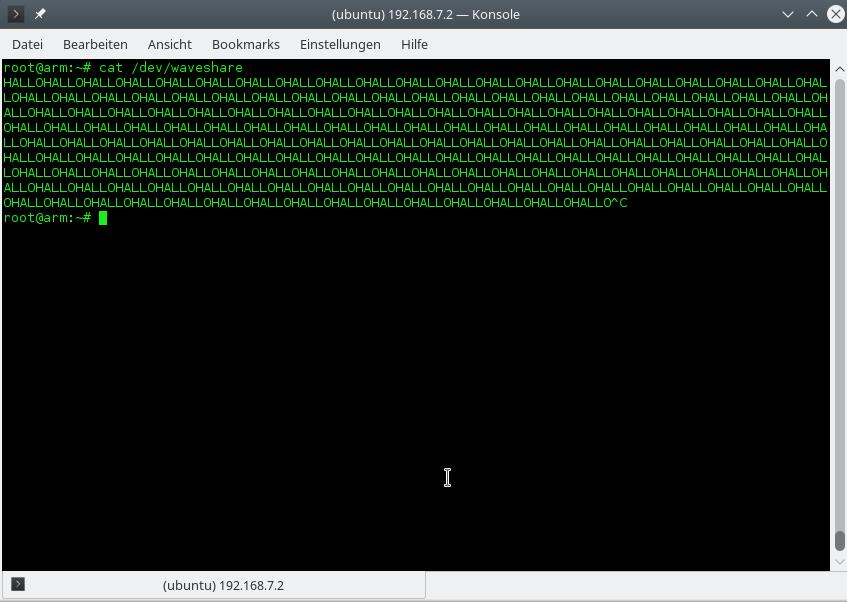
\includegraphics[scale=0.49]{ausgabe_cat_dev_waveshare}
  }
  \caption{Lesen vom Treiber aus dem Userspace}
  \label{pic:cat_read}
\end{figure}

Der Befehl \texttt{echo} ermöglicht es die Funktion \mintinline{c}{waveshare_driver_write()} wie in Abbildung \ref{pic:echo_write} zu triggern. \\

\mintinline{bash}{echo hallo > /dev/waveshare} \\

\begin{figure}[H]
  \centering
  \fbox{
   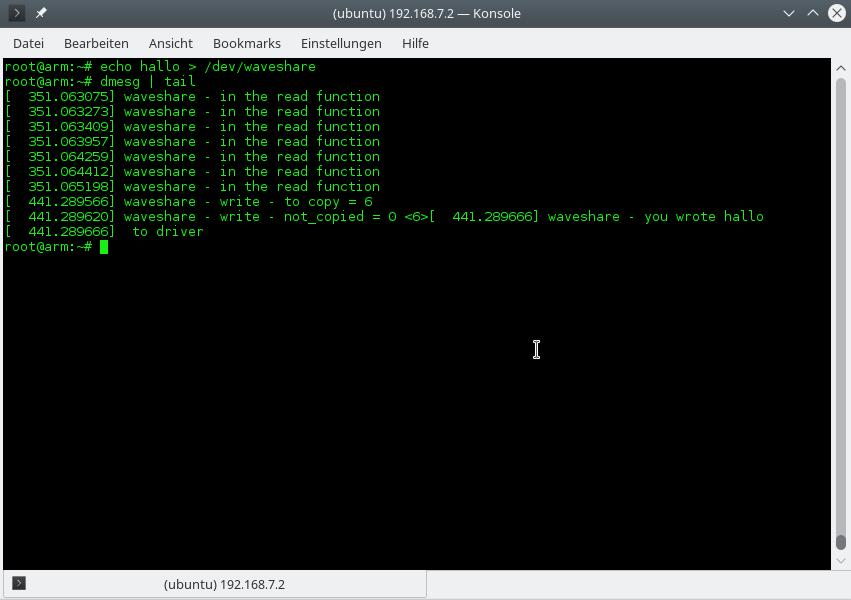
\includegraphics[scale=0.49]{ausgabe_dmesg_echo_dev_waveshare}
  }
  \caption{Schreiben des Treibers aus dem Userspace}
  \label{pic:echo_write}
\end{figure}

\subsection{waveshare\_driver\_poll}  %TODO buch s117/118
Mit dem Systemaufruf \texttt{poll}, hat eine Applikation die Möglichkeit mehrere Quellen, wie zum Beispiel Treiber oder Dateien auf Veränderungen zu überwachen. Die Implementierung auf Seiten des Treibers hat die Aufgabe der Anwendung mitzuteilen, ob mit dem nächsten Aufruf von \texttt{read} Daten gelesen beziehungsweise mit dem nächsten Aufruf von \texttt{write} Daten geschrieben werden können. Es ist möglich, dass die aufrufende Anwendung nach dem Aufruf von \texttt{poll} schlafen gelegt wird, z.B. wenn keine Daten zum Lesen oder Schreiben vorhanden sind. Um dem Betriebssystem mitzuteilen, dass diese Daten für den Treiber nun wieder vorhanden sind, müssen diesem alle Warteschlangen bekannt gegeben werden, die eine solche wartende Applikation enthalten könnten.

In Listing \ref{lst:waveshare_driver_poll}, Zeile 6 und 7 wird gezeigt wie dem Betriebssystem über die Funktion \texttt{poll\_wait()} die Warteschlangen mitgeteilt werden, über die Prozesse aufgeweckt werden, die auf Daten zum Lesen beziehungsweise zum Schreiben warten. 

Die erste if-Abfrage (Zeile 9) prüft das schon bekannte Macro \texttt{READ\_POSSIBLE} das angibt, ob Daten zum Lesen vorhanden sind. Ist dies der Fall, werden Statusbits, in einer Bitmaske verodert, gesetzt. Dabei bedeutet das Flag \texttt{POLLIN}, dass Daten von der Treiberinstanz, die nicht blockiert gelesen werden können. Das Flag \texttt{POLLRDNORM} gibt an, dass Daten zum Lesen verfügbar sind.

Die zweite if-Abfrage (Zeile 12) prüft über das Macro \texttt{WRITE\_POSSIBLE}, ob Daten geschrieben werden dürfen. In diesem Fall werden die Flags in der Bitmaske auf \texttt{POLLOUT} und \texttt{POLLWRNORM} gesetzt, womit angegeben wird, dass Daten geschrieben werden dürfen, ohne dass der Treiber blockiert und dass überhaupt Daten geschrieben werden dürfen. 

Die Bitmaske, die nun besagte Informationen enthält, wird an die aufrufende Anwendung zurückgegeben. 


\begin{listing} [H]
\caption{waveshare\_driver\_poll}
\label{lst:waveshare_driver_poll}
\begin{minted} [xleftmargin=18pt, breaklines, frame=lines, framesep=2mm, fontsize=\footnotesize, linenos] {c}
unsigned int waveshare_driver_poll (struct file *driverinstance, struct poll_table_struct *event_list) {
	
	unsigned int mask = 0;
	
	poll_wait (driverinstance, &wq_read, event_list);
	poll_wait (driverinstance, &wq_write, event_list);

	if (READ_POSSIBLE) {
		mask |= POLLIN | POLLRDNORM;
	}
	if (WRITE_POSSIBLE) {
		mask |= POLLOUT | POLLWRNORM;
	}

	return mask;
}
\end{minted}
\end{listing}


\section{Das Sys-Filesystem} %überschrift anpassen %TODO buch s285
Das Sys-Filesystem sysfs, auch Driver-Filesystem genannt, ist ein virtuelles Filesystem, das im sogenannten Gerätemodell abbildet, wie Prozessoren und Controller mit Peripheriegeräten zusammenhängen. Darin ist nicht nur Hardware verzeichnet, sondern auch zugehörige Software wie zum Beispiel Treiber. Das sysfs löst langfristig das alte Modell des procfs (process filesystem), ein Dateisystem um System- und Prozessinformationen bereitzustellen und zu manipulieren, ab. Für diese Arbeit sollen nur Erweiterungen für das sysfs geschrieben werden. 

Da das sysfs dynamisch aus der erkannten Hardware sowie Treibern generiert wird, ist es als Entwickler nur nötig selbst tätig zu werden, falls ein nicht standardisiertes Bussystem genutzt oder ein neues integriert wird, falls das Energiemanagement der Geräte durch den Treiber gesteuert werden soll, und wenn über Attribute des sysfs Treiber oder Geräte verändert oder ausgelesen werden sollen. Ebenfalls können neue Geräteklassen definiert werden. 

Für den Waveshare-Treiber soll sowohl eine eigene Geräteklasse \glqq waveshare\grqq~definiert werden, sowie Informationsabfrage oder Kontrollzugriff über Attribute des sysfs auf die Hardware. Über solche Kontrollzugriffe, die aus dem Userspace erfolgen, können beispielsweise für Sensoren verschiedene Mess- bzw. Auswertungsintervalle initiiert und kontrolliert werden, ohne die \mintinline{c}{waveshare_driver_read() bzw. waveshare_driver_write()} Funktionen zu ändern oder zu parametrisieren. Für das Display wäre es denkbar über das sysfs verschiedene Funktionen um das Display zu beschreiben, anzubieten, die sich beispielsweise im Zeichensatz (das Display unterstützt auch chinesische Schriftzeichen) oder in der Schriftgröße unterscheiden. Natürlich könnten auch schlicht Informationen über Display und Treiber in Attributen hinterlegt werden. 

Besonders interessant ist hierbei, dass das sysfs selbst im Userspace angesiedelt ist, die Informationen aber vom Kernelmodul erhalten kann, also beispielsweise Sensorergebnisse direkt von einer Messfunktion im Treiber abgerufen werden. Dadurch entfallen einige Punkte, die beim Datenaustausch zwischen User- und Kernelspace in den applikationsgetriggerten Funktionen \texttt{read} und \texttt{write} beachtet werden mussten.

Auf Grund der Probleme bei der Kommunikation mit der Hardware finden sich auch für die Zugriffsfunktionen auf die sysfs-Attribute nur beispielhafte Implementierungen, um Anwendung und Möglichkeiten dieser zusätzlichen Schnittstelle zwischen Treiber bzw. Hardware und Userspace darzustellen.  

%TODO buch s 300...
Zuerst soll eine Funktion für lesenden Zugriff auf ein sysfs-Attribut erstellt werden (Listing \ref{lst:waveshare_sysfs_read}). Dabei wird die Information über die \texttt{sprintf}-Funktion in den entsprechenden Puffer des Lesenden kopiert. Zurückgegeben wird die Anzahl der kopierten Bytes. In dieser Funktion könnte aber auch beispielsweise \texttt{strcpy} oder ähnliches verwendet werden, während in der applikationsgetriggerten Lesefunktion nur der Datenaustausch mittels \texttt{copy\_to\_user()} möglich ist. 
Hier können z.B. Ergebnisse des Treibers auf sehr einfache Weise im Userspace verfügbar gemacht werden.


\begin{listing} [H]
\caption{waveshare\_sysfs\_read}
\label{lst:waveshare_sysfs_read}
\begin{minted} [xleftmargin=18pt, breaklines, frame=lines, framesep=2mm, fontsize=\footnotesize, linenos] {c}
static ssize_t waveshare_sysfs_read (struct device *dev, struct device_attribute *attr, char *buf) {

	char example [] = {"TEST"};

	return sprintf (buf, "%s \n", example); 
}
\end{minted}
\end{listing}


Nun soll noch eine Funktion für schreibenden Zugriff (Listing \ref{lst:waveshare_driver_write}) auf ein solches Attribut erstellt werden. Es ist nicht zwingend notwendig für ein Attribut immer sowohl lesenden als auch schreibenden Zugriff zu realisieren. Attribute, die nur Informationen über Hardware und/oder Treiber zur Verfügung stellen, werden nur mit einer lesenden Zugriffsfunktion verknüpft.
Auch diese Funktion ist nicht sehr spannend, da der Datenaustausch ausschließlich im Userspace stattfindet. Allerdings können so erhaltene Daten im Treiber ausgewertet und weiterverarbeitet werden.


\begin{listing} [H]
\caption{waveshare\_sysfs\_write}
\label{lst:waveshare_sysfs_write}
\begin{minted} [xleftmargin=18pt, breaklines, frame=lines, framesep=2mm, fontsize=\footnotesize, linenos] {c}
static ssize_t waveshare_sysfs_write (struct device *dev, struct device_attribute *attr, const char *buf, size_t size) {
	int val = 0;
	PRINT ("write a number");
	
	val = simple_strtoul (buf, NULL, 10);
	printk (KERN_INFO "You wrote %d \n", val);	
	
	return size;
}
\end{minted}
\end{listing}

Nachdem die Zugriffsfunktionen für das Attribut definiert wurden, werden sie über das Macro \texttt{DEVICE\_ATTR} (Listing \ref{lst:device_attr}) mit einem Attributnamen verknüpft und entsprechende Zugriffsrechte gesetzt. Der erste Parameter des Macros gibt den Namen des Attributs an, für welches die Zugriffsfunktionen definiert wurden, der Zweite beschreibt die Zugriffsrechte (entweder als Zahl oder als Konstantennamen). Die letzten beiden Parameter geben die Adressen der Funktionen für lesenden bzw. schreibenden Zugriff an. Wird nur einer der beiden angeboten, bleibt der jeweilig andere Parameter \texttt{NULL}. Dies muss sich auch in den Zugriffsrechten widerspiegeln. Ist keine Schreibfunktion definiert, darf auch kein schreibender Zugriff zugelassen werden. 


\begin{listing} [H]
\caption{Das DEVICE\_ATTR Macro}
\label{lst:device_attr}
\begin{minted} [xleftmargin=18pt, breaklines, frame=lines, framesep=2mm, fontsize=\footnotesize, linenos] {c}
static DEVICE_ATTR (wav_sysfs, 0644, waveshare_sysfs_read, waveshare_sysfs_write);
\end{minted}
\end{listing}


Zuletzt erfolgt noch das Erstellen der eigenen sysfs-Geräteklasse \glqq waveshare\grqq~sowie die Beauftragung des Gerätemodells, die Attributdatei anzulegen. Dies geschieht in der \mintinline{c}{waveshare_init} Funktion (Listing  \ref{lst:sysfs_class_create}) über \texttt{class\_create} und \texttt{device\_create\_file}.

\begin{listing} [H]
\caption{sysfs Geräteklasse und Attribut erstellen}
\label{lst:sysfs_class_create}
\begin{minted} [xleftmargin=18pt, breaklines, frame=lines, framesep=2mm, fontsize=\footnotesize, linenos] {c}
static int __init waveshare_init (void) {
[...]

	waveshare_class = class_create (THIS_MODULE, WAVESHARE);
	
	if (IS_ERR (waveshare_class)) {
		PRINT ("sysfs class creation failed, no udev support");
		goto free_cdev;
	}
	
    waveshare_dev = device_create (waveshare_class, 
  	   NULL, waveshare_dev_number, NULL, "%s", WAVESHARE);
  	
	if(device_create_file(waveshare_dev, &dev_attr_wav_sysfs)) {
		PRINT ("failed to register attribute file under /dev/waveshare");
	}
	
[...]
}
\end{minted}
\end{listing}

Der Zugriff über die Linux-Kommandozeile auf das sysfs ist in der nachfolgenden Abbildung \ref{pic:sysfs_zugriff} dargestellt.

\begin{figure}[H]
  \centering
  \fbox{
   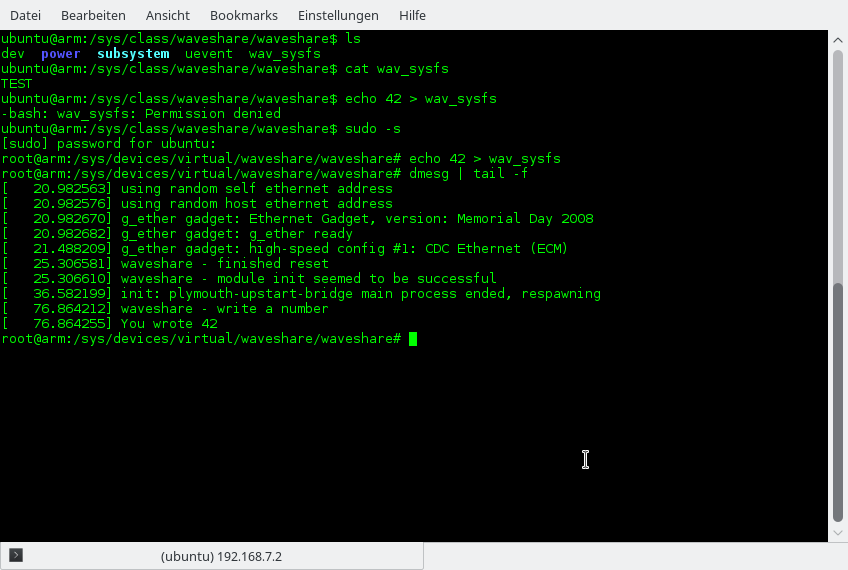
\includegraphics[scale=0.65]{sysfs_zugriff}
  }
  \caption{Zugriff auf das sysfs Attribut}
  \label{pic:sysfs_zugriff}
\end{figure}


